%========================================================
% CHAPTER 3: MODEL FRAMEWORK, DATA, AND METHODOLOGY
%========================================================
\chapter{Model Framework, Data, and Methodology}
\label{chap:framework}

%----------------------------------------------------
\section{Model Framework}
%----------------------------------------------------

\subsection{Baseline CAPM (M1)}

The standard CAPM frames the expected excess return of firm $i$ as:
\begin{equation}
  R_{i,t} - R_{f,t} \;=\; \alpha_i \;+\; \beta_i\bigl(R_{m,t} - R_{f,t}\bigr) \;+\; \varepsilon_{i,t}
  \label{eq:capm}
\end{equation}
where $R_{f,t}$ is the risk-free rate and $R_{m,t}$ is the value-weighted market return. This serves as the M1 benchmark.

\subsection{ESG Level (M2, M2C)}

Model M2 adds the time-varying normalised ESG level $\mathrm{ESG}_{i,t}$ as a return predictor:
\begin{equation}
  R_{i,t} - R_{f,t} \;=\; \alpha_i \;+\; \beta_1\bigl(R_{m,t}-R_{f,t}\bigr) \;+\; \beta_2\,\mathrm{ESG}_{i,t} \;+\; \varepsilon_{i,t}
  \label{eq:m2}
\end{equation}
With entity fixed effects and a time-varying panel, $\beta_2$ is identified purely from \emph{within-firm} ESG variation --- not cross-sectional differences. Model M2C adds a mean-centred interaction $\mathrm{ESG}_{i,t}^c \times (R_{m,t}-R_{f,t})$ to test whether the ESG \emph{level} modulates market beta. The insignificance of this interaction (H6: $t=1.442$, $p=0.149$) provides the null against which the $\Delta$ESG interaction in M6 is contrasted.

\subsection{ESG Change: The Core Model (M6)}

Model M6 replaces the ESG level with its mean-centred month-over-month change $\Delta\mathrm{ESG}_{i,t}^c$ and includes the interaction with the market factor:
\begin{equation}
  R_{i,t} - R_{f,t} \;=\; \alpha_i \;+\; \beta_1\bigl(R_{m,t}-R_{f,t}\bigr) \;+\; \beta_2\,\Delta\mathrm{ESG}_{i,t}^c \;+\; \beta_3\,\Delta\mathrm{ESG}_{i,t}^c\times\bigl(R_{m,t}-R_{f,t}\bigr) \;+\; \varepsilon_{i,t}
  \label{eq:m6}
\end{equation}
Mean-centring $\Delta\mathrm{ESG}$ before forming the interaction term resolves the multicollinearity inherent in interaction models, confirmed by a max VIF of 1.075 (see Section~\ref{sec:diagnostics}). $\beta_2$ tests whether ESG improvements are contemporaneously priced (H3). $\beta_3$ tests whether ESG change modulates systematic risk (H5) --- the Beta Amplification Paradox.

\subsection{ESG Momentum: Predictive Specification (P1--P3)}

Three specifications test whether lagged $\Delta\mathrm{ESG}$ predicts next-month returns:
\begin{equation}
  R_{i,t} - R_{f,t} \;=\; \alpha_i \;+\; \sum_{k}\gamma_k f_{k,t} \;+\; \gamma_6\,\Delta\mathrm{ESG}_{i,t-1}^c \;+\; \varepsilon_{i,t}
  \label{eq:momentum}
\end{equation}
P1 includes only entity and year fixed effects; P2 adds Mkt-RF; P3 adds the full Fama-French five-factor set. A significant $\gamma_6$ in P3 (H4) establishes ESG momentum as an independent predictive channel net of all standard risk factors.

\subsection{Component-Level Decomposition}

To test whether the aggregate ESG signal or its sub-components drive results, we re-estimate M6 and P3 replacing $\Delta\mathrm{ESG}^c$ with $\Delta E^c$, $\Delta S^c$, and $\Delta G^c$ separately. If the market prices the holistic rating rather than its individual dimensions, component-level regressions should yield insignificant coefficients even when the aggregate is significant.

\subsection{Economic Intuition}

Each coefficient has a clear economic story. $\beta_2$ reflects the information channel: an ESG revision signals changes in regulatory exposure, governance quality, or operational sustainability that the market prices rapidly. $\beta_3$ tests whether firms in ESG transition decouple from or amplify market co-movement. $\gamma_6$ tests whether ESG information is fully absorbed on impact or whether gradual institutional rebalancing generates persistent predictability. The Fama-MacBeth cross-sectional tests (H2) separately ask whether the level of ESG commands a cross-sectional risk premium independent of within-firm dynamics.

%----------------------------------------------------
\section{Data}
%----------------------------------------------------

\subsection{Sample and Variables}

The sample consists of 479 S\&P 500 constituent firms with continuous Sustainalytics ESG coverage over February 2015 to December 2024, yielding \textbf{56,656 firm-month observations}. Monthly total returns are from CRSP; Fama-French five-factor returns and the risk-free rate are from Kenneth French's data library. Sectors follow the eleven-sector GICS classification.

Sustainalytics scores are risk measures: higher raw scores indicate greater unmanaged ESG exposure. All scores are normalised to $[0,1]$ with direction inverted so that higher $\mathrm{ESG}_{i,t}$ denotes lower ESG risk (better ESG). The panel mean is 0.586 (SD $\approx$ 0.19). Industrials and Financials each contribute 74 firms; Consumer Discretionary contributes 46.

\begin{figure}[H]
  \centering
  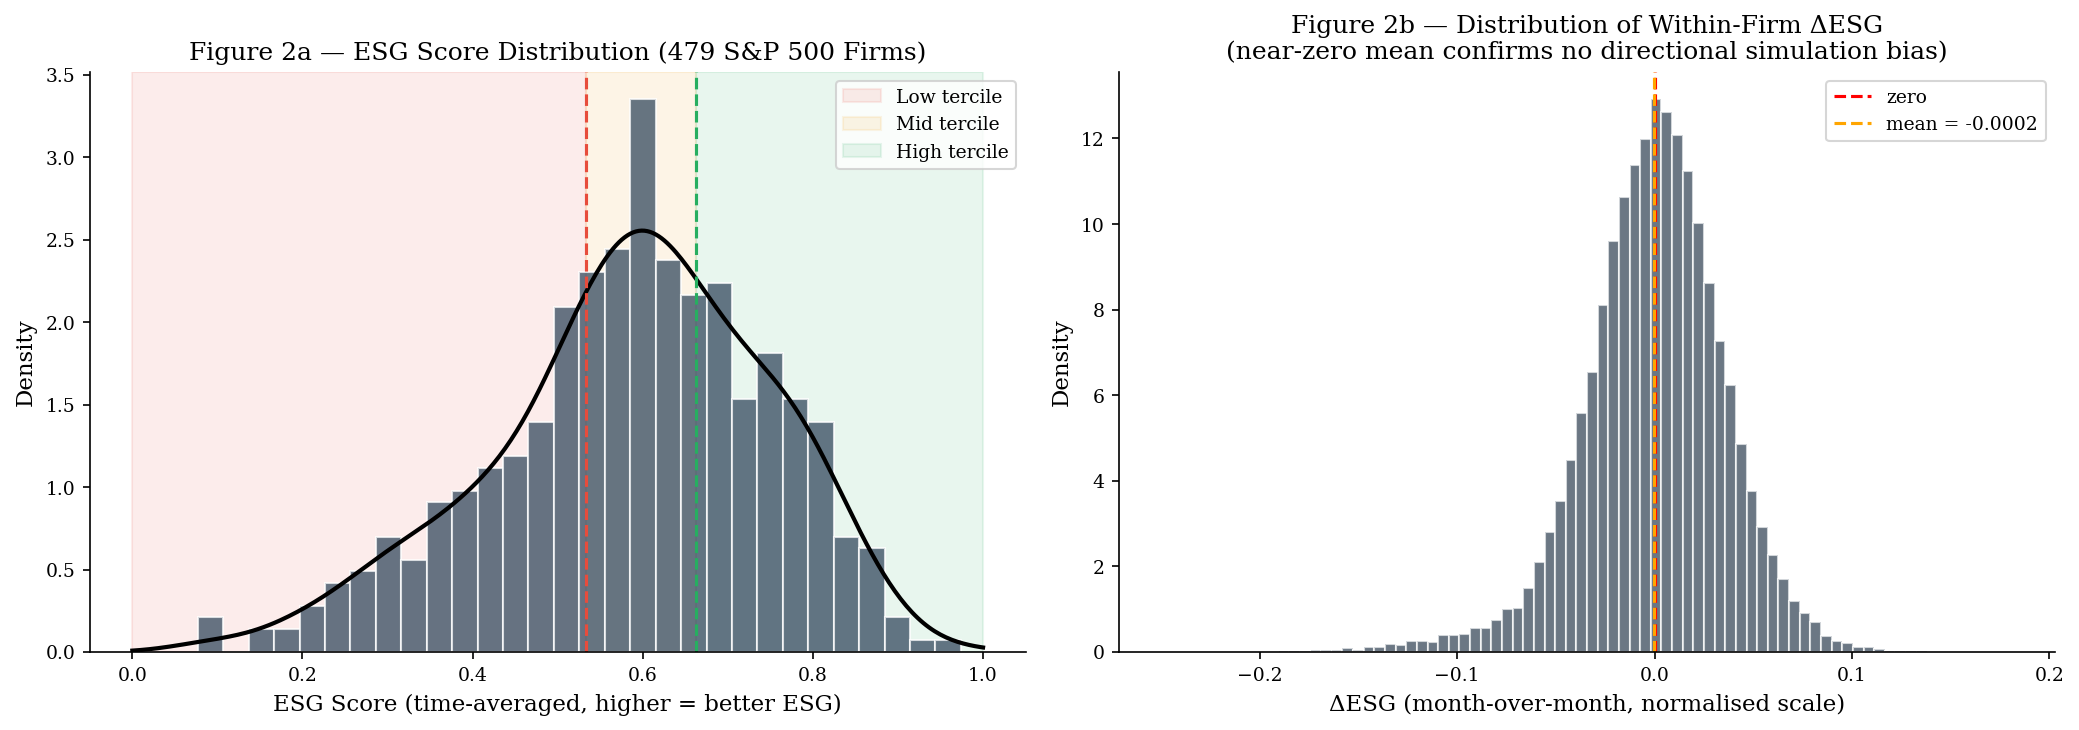
\includegraphics[width=\textwidth]{../Pictures/fig2_esg_dynamics.png}
  \caption{\textbf{Figure 2 --- ESG score distribution vs. $\Delta$ESG distribution }
  Diagnostics for Simulated ESG Dynamics.}
  Diagnostic views of the interpolated ESG panel, including the distribution of within-firm $\Delta\mathrm{ESG}_{i,t}$ and sector-level heterogeneity in ESG evolution. The near-symmetry around zero indicates no directional interpolation bias.}
  \label{fig:esg_distribution}
\end{figure}



\subsection{Time-Varying ESG Panel via Stochastic Interpolation}
\label{sec:stochastic_modeling}

Given that statutory ESG disclosures are typically restricted to annual intervals, we address the resulting temporal coarseness by constructing a high-frequency monthly panel via a multi-factor stochastic framework. Unlike deterministic interpolation, which artificially suppresses volatility and biases standard errors in fixed-effects estimations, our approach preserves the stylized empirical facts of ESG data: high persistence, sector-level co-movement, and tail-risk sensitivity.

The latent ESG score for firm $i$ in sector $s$ at time $t$, denoted by $\mathcal{E}_{i,t}$, is decomposed into four structural components:
\begin{equation}
  \mathcal{E}_{i,t} = \underbrace{\Theta_i(t)}_{\text{Secular Trend}} + \underbrace{X_{i,t}}_{\text{OU Process}} + \underbrace{\eta_{s(i),t}}_{\text{Sector Factor}} + \underbrace{C_{i,t}}_{\text{Controversy Shock}} + \epsilon_{i,t}
\end{equation}
where $\epsilon_{i,t} \sim \mathcal{N}(0, \sigma_\epsilon^2)$ represents idiosyncratic white noise. The components are defined as follows:
\begin{enumerate}
  \item \textbf{Secular trend ($\Theta_i$):} To reflect the broad improvement in ESG reporting quality and corporate adoption, we specify a linear drift $\Theta_i(t) = \bar{E}_i[1 + \gamma(t - t_0)]$, where $\gamma$ is calibrated to a total panel drift of $+8$ points, consistent with S\&P 500 longitudinal averages.

  \item \textbf{Mean-reverting dynamics ($X_{i,t}$):} Short-term deviations from the long-run mean follow an Ornstein-Uhlenbeck (OU) process:
  \begin{equation}
    dX_{i,t} = -\kappa X_{i,t}\,dt + \sigma_i\,dW_{i,t}
  \end{equation}
  The mean-reversion speed $\kappa$ is set to target a half-life of approximately 12 months. We further model $\sigma_i$ as a decreasing function of the baseline score $\bar{E}_i$, reflecting the empirical regularity that highly rated ESG leaders exhibit lower rating volatility than laggards.

  \item \textbf{Sectoral co-movement ($\eta_{s,t}$):} Sector-specific shocks, such as regulatory shifts or industry-wide technological disruptions, follow a first-order autoregressive process, $\eta_{s,t} = \rho\eta_{s,t-1} + \xi_{s,t}$, ensuring that firms within the same GICS sector share common latent variation.

  \item \textbf{Controversy events ($C_{i,t}$):} Negative ESG externalities are modeled as Poisson arrivals $\Pi(\lambda)$ with monthly intensity $\lambda = 0.04$. Each event $j$ induces a discrete jump $J_{i,j} \sim \mathcal{N}(\mu_c, \sigma_c)$, which then decays toward the mean through the OU mechanism, simulating reputational recovery.
\end{enumerate}

To maintain internal consistency across the environmental ($E$), social ($S$), and governance ($G$) pillars, sub-scores are generated using a Cholesky decomposition of the empirical correlation matrix $\mathbf{\Omega}$:
\begin{equation}
  \begin{pmatrix} E \\ S \\ G \end{pmatrix}_{i,t} = \mathbf{L}\mathbf{Z}_{i,t}, \qquad \text{where } \mathbf{L}\mathbf{L}^{\top} = \mathbf{\Omega}
\end{equation}
where $\mathbf{Z}_{i,t}$ is a vector of independent standard normal shocks. This construction ensures that the synthetic panel reproduces both the aggregate ESG distribution and the cross-pillar dependence structure documented in the sustainable finance literature.

Figure~\ref{fig:esg_trajectories} illustrates the resulting within-firm dynamics for twelve representative firms.

\begin{figure}[H]
  \centering
  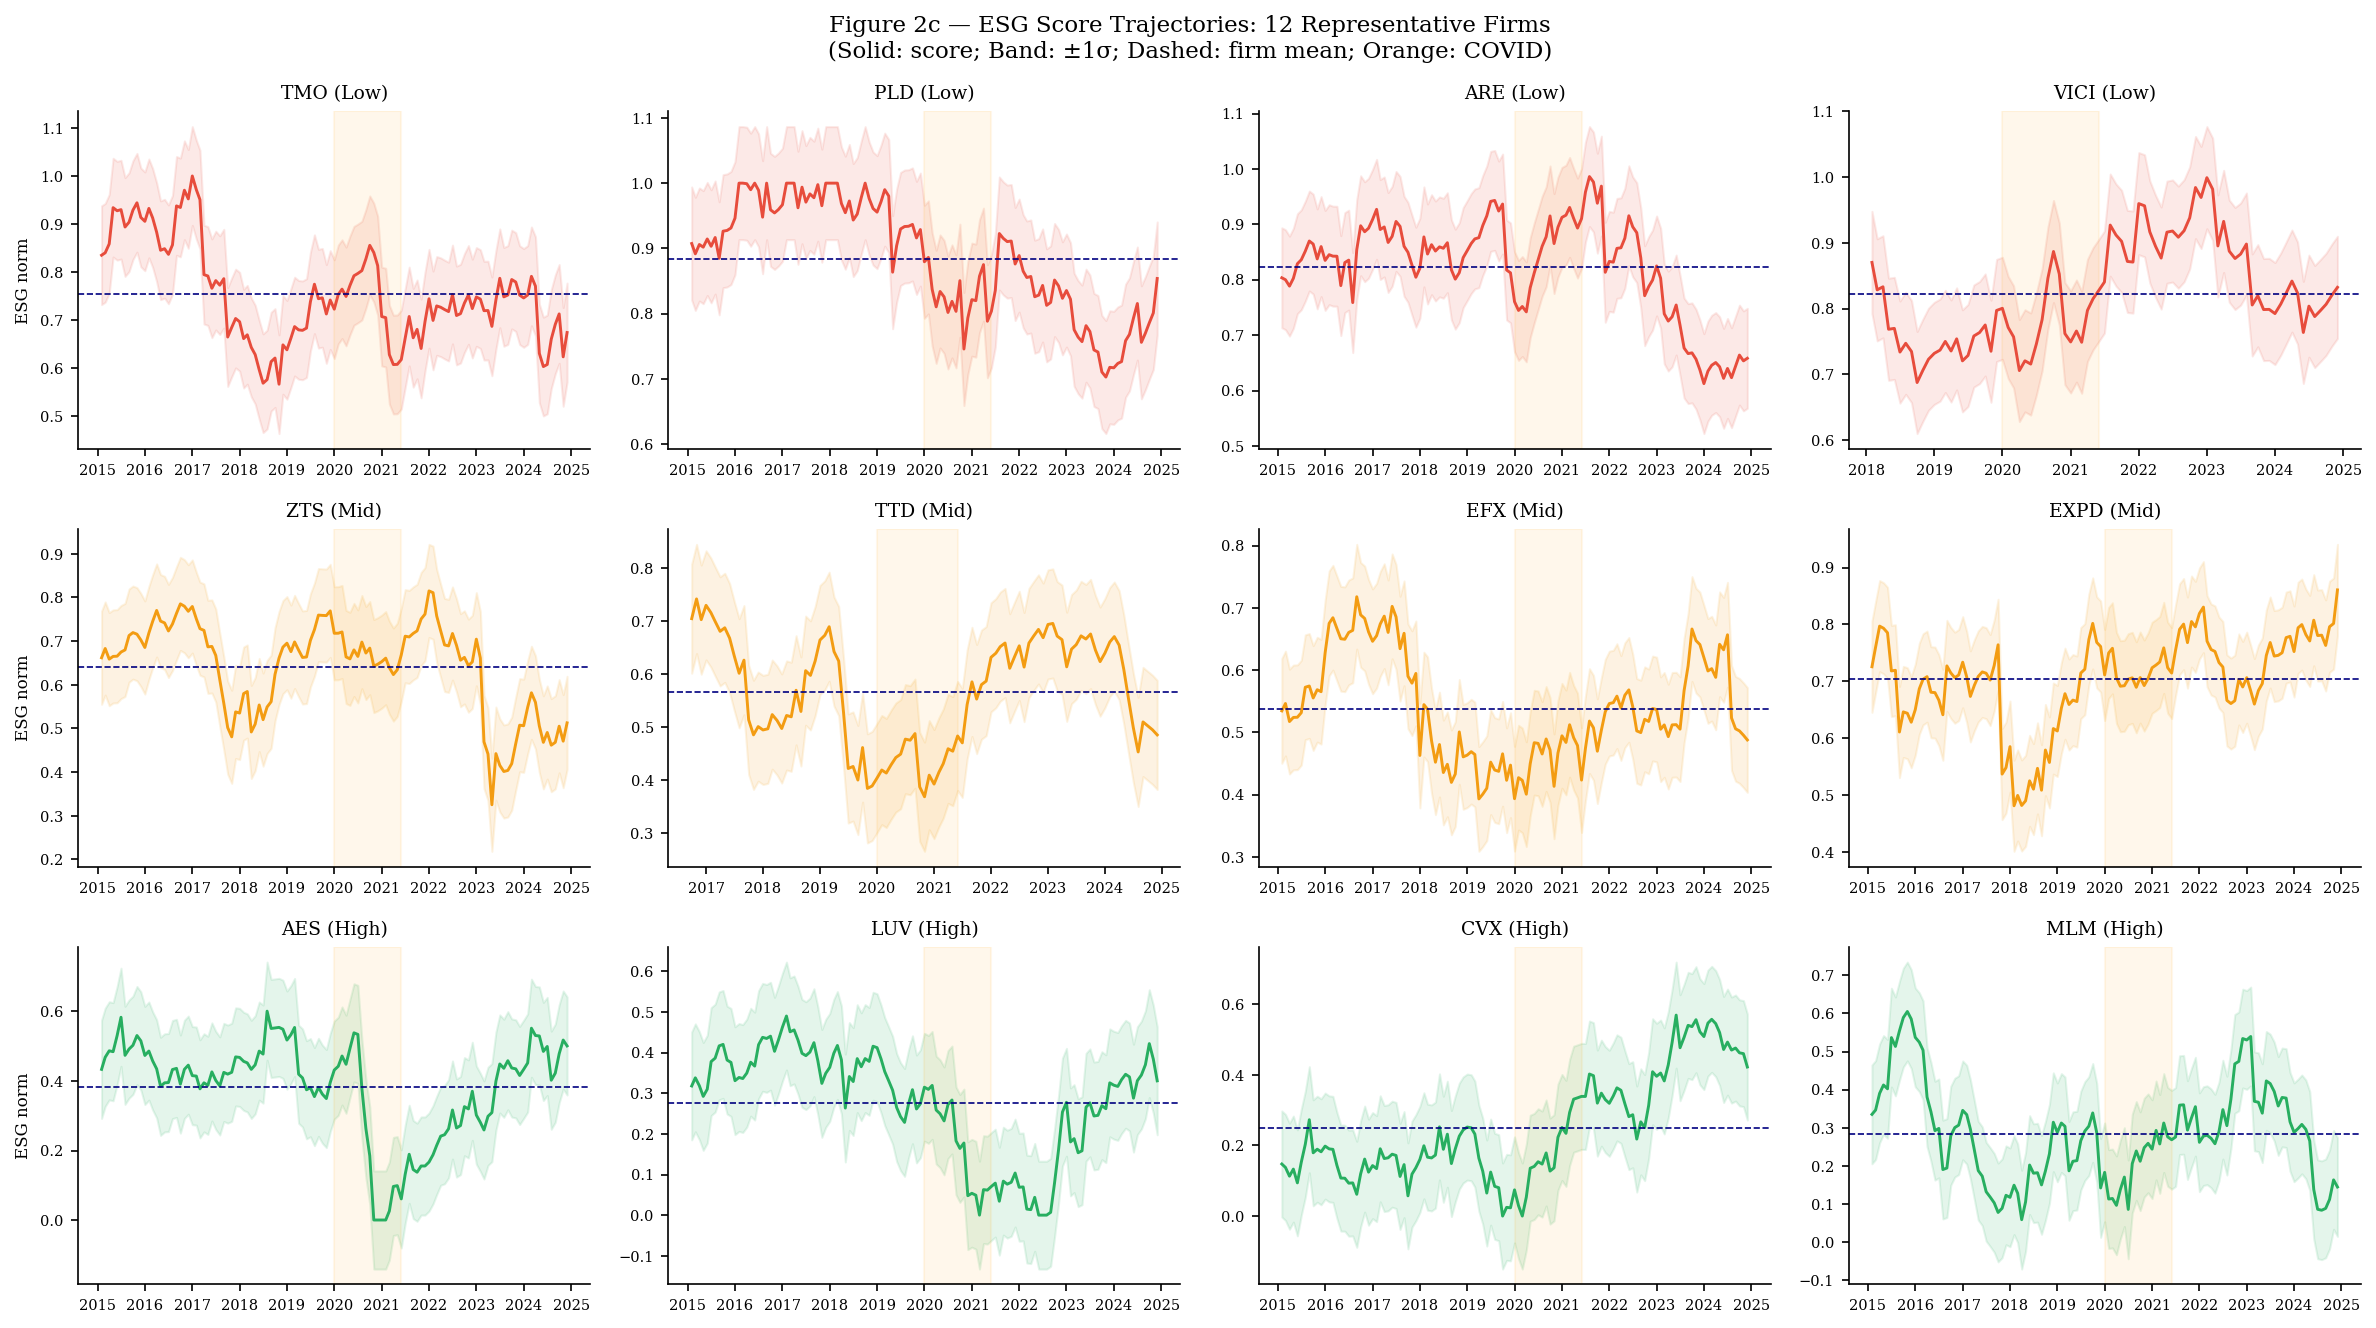
\includegraphics[width=\textwidth]{Pictures/fig2c_esg_trajectories.png}
  \caption{\textbf{Figure 2b --- Time-Varying ESG Score Trajectories.}
  Monthly normalised ESG score for twelve representative firms sampled across ESG terciles and GICS sectors. Solid line: score. Shaded band: $\pm 1\sigma$. Dashed line: firm mean. Orange shading: COVID-19 period (Jan 2020--Jun 2021). Within-firm variation is the identifying variation for M2 and M6.}
  \label{fig:esg_trajectories}
\end{figure}

The $\Delta\mathrm{ESG}$ distribution shown in Figure~\ref{fig:esg_distribution} is approximately symmetric around zero, ruling out directional interpolation bias.


%----------------------------------------------------
\section{Methodology}
%----------------------------------------------------

\subsection{Pre-Regression Diagnostic Pipeline}
\label{sec:diagnostics}

All model specification choices are driven by a pre-regression diagnostic pipeline rather than arbitrary convention. Table~\ref{tab:diagnostics} summarises the four tests and their implications.

\begin{table}[H]
  \centering
  \caption{Pre-Regression Diagnostic Tests. Tests are run on the full 56,656-observation panel prior to any hypothesis testing.}
  \label{tab:diagnostics}
  \small
  \begin{tabular}{l>{\raggedright\arraybackslash}p{3.0cm}cc>{\raggedright\arraybackslash}p{4.1cm}}
    \toprule
    & Test & Statistic & $p$-value & Implication \\
    \midrule
    D1 & Hausman (Mundlak)      & $\chi^2 = 12.044$ & $<0.001$ & FE preferred over RE \\
    D2 & Pesaran CD             & $129.867$         & $<0.001$ & Cross-sectional dependence present; clustered SEs used \\
    D3 & Wooldridge AR(1)       & $F = 87.194$      & $<0.001$ & Serial correlation present; Newey-West SEs applied \\
    D4 & VIF (M6 regressors)    & max VIF $= 1.075$ & ---      & Mean-centering $\Delta$ESG resolves collinearity \\
    \bottomrule
  \end{tabular}
  \smallskip\\
  \footnotesize \textit{Notes}: D1 rejects random effects in favour of fixed effects ($p<0.001$). D2 and D3 jointly justify both firm-clustered and Newey-West (12-lag) standard errors. D4 confirms that mean-centring $\Delta\mathrm{ESG}^c$ before interaction construction keeps all VIFs below the conventional threshold of 5.
\end{table}

\subsection{Panel Fixed Effects Regression}

All panel specifications include firm and year fixed effects, estimated by within-group demeaning. The Hausman test (D1) mathematically justifies fixed over random effects. Standard errors are clustered at the firm level (D2) and, where serial correlation is a concern, Newey-West with twelve lags is applied (D3). The first observation per firm is dropped in $\Delta\mathrm{ESG}$ specifications to avoid using returns without valid lagged ESG changes.

\subsection{Fama-MacBeth Cross-Sectional Regressions}

Each month $t$, excess returns are regressed cross-sectionally on full-period OLS beta and time-varying ESG level. The time series of monthly ESG slope coefficients is averaged and tested using Newey-West standard errors with twelve lags \citep{newey1987simple}, testing whether ESG level commands a cross-sectional risk premium independently of within-firm dynamics.

